\documentclass[11pt,a4paper]{article}

% Packages
\usepackage{amsmath,amssymb,amsfonts}
\usepackage{geometry}
\usepackage{tikz}
\usetikzlibrary{decorations.pathmorphing,arrows.meta,positioning,calc,3d}
\usepackage{enumitem}
\usepackage{graphicx}
\usepackage[american]{circuitikz}
\usetikzlibrary{arrows.meta}

% تنظیم ابعاد و یکسان‌سازی ضخامت مقاومت با سیم‌های مدار
\ctikzset{
    bipoles/resistor/height=0.22,
    bipoles/resistor/width=0.45,
    bipoles/thickness=1
}

\usepackage{xepersian}

% Page Setup
\geometry{
    top=2cm,
    bottom=2cm,
    left=2cm,
    right=2cm
}

% Fonts Setup (تنظیم فونت‌ها بر اساس سیستم خودتان)
\settextfont[Scale=1.05]{XB Niloofar}
%\setlatintextfont[Scale=0.95]{Times New Roman}
\defpersianfont\nastaliq[Scale=1.5]{IranNastaliq}

\setlength{\parindent}{0pt}
\setlength{\parskip}{6pt}

\begin{document}

% ==================== PAGE 1 ====================
\begin{minipage}[t]{0.15\textwidth}
    \vspace{0pt}
    % در صورت داشتن فایل لوگوی دانشگاه، خط زیر را از حالت کامنت خارج کنید:
     
\includegraphics[width=2.2cm]{sut.jpg}
    %\begin{tikzpicture}[scale=0.7]
     %   \draw[thick] (0,0) circle (1.2cm);
     %   \draw (0,0) circle (0.9cm);
     %   \node at (0,0.2) {\tiny دانشگاه صنعتی شریف};
     %   \node at (0,-0.3) {\tiny ۱۳۴۴};
    %\end{tikzpicture}
\end{minipage}%
\begin{minipage}[t]{0.85\textwidth}
    \vspace{0pt}
    \centering
    {\nastaliq امتحان میان‌ترم اول درس الکترومغناطیس ۲ - پاییز ۱۴۰۵} \\[12pt]
    {\nastaliq دانشکده فیزیک - دانشگاه صنعتی شریف} \\[12pt]
    {\nastaliq دوشنبه ۱۱ آبان ۱۴۰۵ ساعت ۱۶:۳۰}
\end{minipage}

\vspace{4pt}
\hrule height 0.8pt
\vspace{6pt}

\begin{itemize}[label=$\bullet$, rightmargin=0.5cm, itemsep=2pt]
    \item لطفا نام، نام خانوادگی و شماره‌ی دانشجویی خود را بر روی پاسخ‌نامه مرقوم فرمایید.
    \item مدت امتحان ۲ ساعت است.
    \item امتحان شامل ۲ سوال است. لطفا هر سوال را در برگه‌ی مجزا جواب دهید.
    \item امتیاز سوال‌ها به صورت زیر است: سوال یک ۲۰ امتیاز سوال دو ۲۲ امتیاز
    \item کل سوالات ۴۲ نمره دارد. کسب ۴۰ نمره کفایت می‌کند.
    \item میان‌ترم اول ۴ نمره پایانی را تشکیل می‌دهد. \hfill با احترام، شانت باغرام
\end{itemize}

\vspace{4pt}
\hrule height 0.8pt
\vspace{10pt}

\underline{\textbf{\textit{سوال ۱) سوال‌های کوتاه: سوال‌های زیر را لطفا مختصر جواب دهید!}}}

\vspace{4pt}
۱-۱) توضیح دهید که چگونه ماکسول با استفاده از ایده‌ی پایستگی بار، معادله‌ی آمپر را تصحیح و مفهوم جریان جابه‌جایی را تعریف کرد.

۱-۲) سه آزمایش فارادی را که در زیر به صورت طرح‌واره نشان داده شده است، شرح دهید:

\vspace{6pt}
\begin{latin}
\begin{center}
\begin{circuitikz}[
    >=Stealth,
    line width=0.9pt
]

% ماکروی مشترک برای ناحیه میدان مغناطیسی و حلقه مدار
\newcommand{\drawsetup}[2]{
    % کادر ناحیه میدان مغناطیسی (بدون رنگ خاکستری)
    \draw (#1,0) rectangle (#1+3,3);
    \node[anchor=south west, font=\bfseries] at (#1+0.1, 0.1) {#2};

    % حلقه رسانا و مقاومت با ضخامت و استایل یکسان
    \draw (#1+3.8, 1.9) -- (#1+1.6, 1.9) -- (#1+1.6, 0.9) -- (#1+3.8, 0.9);
    \draw (#1+3.8, 1.9) to[R] (#1+3.8, 0.9);

    % فلش جهت جریان ساعتگرد و برچسب I
    \draw[->, line width=0.8pt] (#1+3.25, 1.68) arc[start angle=75, end angle=-75, radius=0.29];
    \node at (#1+3.12, 1.4) {$I$};
}

% --- شکل (a) ---
\drawsetup{0}{B \normalfont(in)}
\draw[->, line width=0.8pt] (4.15, 1.4) -- node[above=2pt] {$v$} (4.75, 1.4);
\node at (1.5, -0.5) {(a)};

% --- شکل (b) ---
\drawsetup{5.6}{B \normalfont(in)}
\draw[->, line width=0.8pt] (5.5, 1.4) -- node[above=2pt] {$v$} (4.9, 1.4);
\node at (7.1, -0.5) {(b)};

% --- شکل (c) ---
\drawsetup{10.2}{B}
\node at (11.7, -0.5) {(c)};

% فلش منحنی و متن Changing magnetic field
\node[align=center] (cmf) at (9.2, -1.0) {Changing\\magnetic field};
\draw[->, line width=0.8pt] (10.6, 0.15) to[out=-75, in=10] (9.6, -0.25) -- (9.35, -0.6);

\end{circuitikz}
\end{center}
\end{latin}

۱-۳) جریان قطبش $\vec{J}_p$ را به دلیل تغییر قطبش الکتریکی به دست آورید و نشان دهید که چگونه در رابطه‌ی پایستگی زیر صدق می‌کند. $\rho_b$ چگالی بار مقید است.
\[
\frac{\partial \rho_b}{\partial t} + \vec{\nabla} \cdot \vec{J}_p = 0
\]

۱-۴) بردار پوئینتینگ $\vec{S}$ را تعریف کنید و نشان دهید که در صورت صفر بودن کار انجام شده بر بار، بردار پوئینتینگ در رابطه پایستگی انرژی به صورت روبرو صدق می‌کند: $\frac{\partial u_{EM}}{\partial t} = -\vec{\nabla} \cdot \vec{S}$.

توجه داشته باشید که $u$ چگالی انرژی است. $\left( u_{EM} = \frac{1}{2} \left( \epsilon_0 |\vec{E}|^2 + \frac{1}{\mu_0} |\vec{B}|^2 \right) \right)$

۱-۵) به صورت کیفی توضیح دهید که چگونه یک کره آهنی باردار با بار $Q$ که دارای مغناطش ثابت $M$ در یک راستای مشخص است، می‌تواند شروع به چرخش کند اگر:

الف) مغناطش آن را با زمان کاهش دهیم. - \lr{Demagnetization}

ب) بار الکتریکی را به طریق مناسب از آن خارج کنیم. - \lr{Discharge}

\vspace{4pt}
توجه کنید که کره ابتدا ساکن است و می‌تواند آزادانه حول محور مغناطش بچرخد.

% ==================== PAGE 2 ====================
\newpage

\underline{\textbf{\textit{سوال ۲) تکانه زاویه میدان الکترومغناطیس}}}

\vspace{8pt}
استوانه‌ای عایق الکتریکی، بی‌نهایت بلند و به شعاع $b$ (مطابق شکل پایین صفحه) دارای مغناطش یکنواخت
\[
\vec{M} = M\hat{z}
\]
است. دو پوسته استوانه‌ای رسانای نازک، به شعاع‌های $a$ و $c$، با این استوانه هم‌محورند، به طوری که
\[
a < b < c
\]
پوسته داخلی دارای بار الکتریکی بر واحد طول $+\lambda$ و پوسته خارجی دارای بار الکتریکی بر واحد طول $-\lambda$ است. پوسته داخلی درون ماده مغناطیده قرار دارد. هر دو پوسته در ابتدا ساکن‌اند. گذردهی الکتریکی را در همه جا برابر با $\epsilon_0$ فرض کنید. از تابش، اثرات انتهایی و میدان‌های مغناطیسی ناشی از چرخش بعدی پوسته‌ها نیز صرف‌نظر کنید.

\vspace{6pt}
الف) میدان‌های الکتریکی و مغناطیسی را در تمام نواحی به دست آورید.

ب) تکانه زاویه‌ای الکترومغناطیسی بر واحد طول را نسبت به محور استوانه محاسبه کنید.

ج) مغناطش استوانه به آرامی (تغییرات کُند) و به طور همگن مکانی به صفر کاهش می‌یابد. با استفاده از قانون فارادی، میدان الکتریکی القایی را برحسب فاصله از محور استوانه، $s$، به دست آورید.

د) گشتاور بر واحد طول وارد بر هر پوسته و تکانه زاویه‌ای بر واحد طول منتقل شده به آن را محاسبه کنید. نشان دهید مجموع تکانه‌های زاویه‌ای منتقل شده به دو پوسته، برابر با تکانه زاویه‌ای الکترومغناطیسی اولیه است. توجه کنید که دو پوسته می‌توانند آزادانه و بدون اصطکاک حول محور مشترک بچرخند و هیچ گشتاور مکانیکی از طرف ماده عایق به آن‌ها وارد نمی‌شود.»

\vspace{16pt}
\begin{latin}
\begin{center}
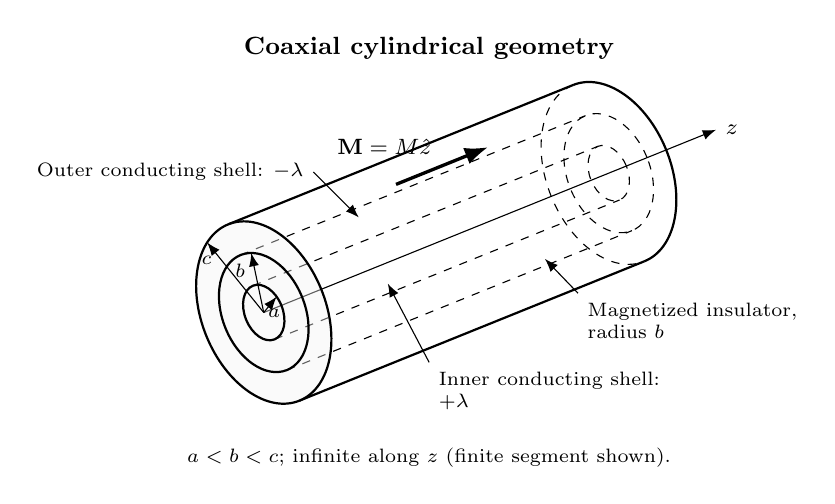
\begin{tikzpicture}[scale=1.05, >=Latex]
    % Title
    \node[font=\small\bfseries] at (2, 3.2) {Coaxial cylindrical geometry};

    % Axis vector parameters:tilt angle 22 degrees, length 4.5
    \def\ang{22}
    \def\L{4.5}
    \pgfmathsetmacro{\dx}{\L*cos(\ang)}
    \pgfmathsetmacro{\dy}{\L*sin(\ang)}

    % Front face center at (0,0)
    % Radii: a=0.35, b=0.75, c=1.15 (ellipses rotated by \ang)
    
    % Back face ellipses (partially visible/dashed)
    \begin{scope}[shift={(\dx,\dy)}, rotate=\ang]
        \draw[thick] (-90:0.75 and 1.15) arc (-90:90:0.75 and 1.15);
        \draw[dashed, thin] (90:0.75 and 1.15) arc (90:270:0.75 and 1.15);
        
        \draw[dashed, thin] (0,0) ellipse (0.5 and 0.75);
        \draw[dashed, thin] (0,0) ellipse (0.23 and 0.35);
    \end{scope}

    % Connecting lines along cylinder length
    % Outer shell c
    \draw[thick] ({-1.15*sin(\ang)}, {1.15*cos(\ang)}) -- ++(\dx,\dy);
    \draw[thick] ({1.15*sin(\ang)}, {-1.15*cos(\ang)}) -- ++(\dx,\dy);

    % Middle insulator b
    \draw[dashed, thin] ({-0.75*sin(\ang)}, {0.75*cos(\ang)}) -- ++(\dx,\dy);
    \draw[dashed, thin] ({0.75*sin(\ang)}, {-0.75*cos(\ang)}) -- ++(\dx,\dy);

    % Inner shell a
    \draw[dashed, thin] ({-0.35*sin(\ang)}, {0.35*cos(\ang)}) -- ++(\dx,\dy);
    \draw[dashed, thin] ({0.35*sin(\ang)}, {-0.35*cos(\ang)}) -- ++(\dx,\dy);

    % Central z-axis
    \draw[->, thin] (0,0) -- ({(\L+1.4)*cos(\ang)}, {(\L+1.4)*sin(\ang)}) node[right, font=\footnotesize] {$z$};

    % Front face ellipses
    \begin{scope}[rotate=\ang]
        \draw[thick, fill=gray!10, fill opacity=0.4] (0,0) ellipse (0.75 and 1.15);
        \draw[thick] (0,0) ellipse (0.5 and 0.75);
        \draw[thick] (0,0) ellipse (0.23 and 0.35);

        % Radius arrows a, b, c
        \draw[->, thin] (0,0) -- (20:0.23 and 0.35) node[below, font=\scriptsize, pos=0.8] {$a$};
        \draw[->, thin] (0,0) -- (75:0.5 and 0.75) node[left, font=\scriptsize, pos=0.7] {$b$};
        \draw[->, thin] (0,0) -- (115:0.75 and 1.15) node[left, font=\scriptsize, pos=0.75] {$c$};
    \end{scope}

    % Magnetization vector M
    \draw[->, very thick] (1.6, 1.55) -- ++({1.2*cos(\ang)}, {1.2*sin(\ang)}) node[midway, above left, font=\footnotesize] {$\mathbf{M} = M\hat{z}$};

    % Labels and pointers
    \node[font=\scriptsize, anchor=east] (outer_lbl) at (0.6, 1.7) {Outer conducting shell: $-\lambda$};
    \draw[->, thin] (outer_lbl.east) -- (1.15, 1.15);

    \node[font=\scriptsize, align=left, anchor=west] (mag_lbl) at (3.8, -0.1) {Magnetized insulator,\\radius $b$};
    \draw[->, thin] (mag_lbl.north west) -- (3.4, 0.65);

    \node[font=\scriptsize, align=left, anchor=west] (inner_lbl) at (2.0, -0.95) {Inner conducting shell:\\$+\lambda$};
    \draw[->, thin] (inner_lbl.north west) -- (1.5, 0.35);

    % Bottom caption
    \node[font=\scriptsize] at (2, -1.75) {$a < b < c$; infinite along $z$ (finite segment shown).};
\end{tikzpicture}
\end{center}

\vfill
{\small
``Inspiration exists, but it has to find you working.''\\
\textbf{Pablo Picasso}
}
\end{latin}

\end{document}